
\chapter{Hyperbolic System}\label{chap2}


\section{Introduction}\label{chap2:sec2.1}
In this\pageoriginale section we define a first order hyperbolic
system and its characteristic cruves. We study the characteristic form
of a first order hyperbolic system and apply these ideas to the
equations of hydrodynamics.

Consider a system of $n$ equations given by 
\begin{equation*}
\frac{\partial u_i}{\partial t} + \sum\limits^n_{j=1} a_{ij} (u,x,t)
\frac{\partial u_j}{\partial x} = 0, \quad 1 \leq i \leq n. 
\tag{2.1}\label{eq2.1}
\end{equation*}
By setting
\begin{equation*}
\left.
\begin{aligned}
A & = (a_{ij}), \; 1 \leq i, j\leq n\\
U^T & = (u_1 (x), \ldots, u_n(x))
\end{aligned}
\right\} \tag{2.2}\label{eq2.2}
\end{equation*}
we can write (\ref{eq2.1}) in the vector form as
\begin{equation*}
\frac{\partial U}{\partial t} + A(U, x,t) \frac{\partial U}{\partial
  x} = 0.\tag{2.3}\label{eq2.3}
\end{equation*}

Given a system of equations of the form (\ref{eq2.1}) or equivalently (\ref{eq2.3})
with $A$ depending on $x$, $U$ and $t$, we look for a curve $C$
parametrised by $x = x(s)$, $t=t(s)$ so that along $C$ some kind of
differential relationship holds for $U$. 

\section{Characteristic form of a first order hyperbolic
  system}\label{chap2:sec2.2}

In the study of first order systems as in (\ref{eq2.1}), the eigenvalues and
eigenvectors of the matrix $A$ play an important role. We start our
discussion with the following:

\setcounter{Definition}{0}
\begin{Definition}\label{chap2:def2.1}
The system of equations (\ref{eq2.1}) is strictly hyperbolic if, and only if,
for all values of its arguments, the matrix $A$ always has $n$ real
and distinct eigenvalues.
\end{Definition}

We\pageoriginale will henceforth consider only such systems which are
strictly hyperbolic.

\setcounter{remark}{0}
\begin{remark}\label{chap2:rem2.1}
If $A$ depends on $U$ then the system of equations is non-linear.
\end{remark}

Let us now study the various cases involved in equation (\ref{eq2.3}).

\medskip
\noindent{\textbf{Case (i).}} Let us assume that the matrix $A$ is
constant. Let $p^T$ be a left-eigen vector of $A$, i.e.
\begin{equation*}
p^T A = \lambda p^T. \tag{2.4}\label{eq2.4}
\end{equation*}
Since $A$ is a constant matrix, $\lambda$ is a constant and $p^T$ is a
constant row-vector. Using these facts and multiplying (\ref{eq2.3}) on the
left by $p^T$, we get 
\begin{equation*}
\frac{\partial}{\partial t} (p^TU) + \lambda \frac{\partial}{\partial
  x}(p^TU) = 0. \tag{2.5}\label{eq2.5}
\end{equation*}

If we now define a plane curve $C$ (which is easily seen to be a
straight line in this case) by
\begin{equation*}
\frac{dt}{ds} = 1; \; \frac{dx}{ds} = \lambda \tag{2.6}\label{eq2.6}
\end{equation*}
or, equivalently,
\begin{equation*}
\frac{dx}{dt} = \lambda \tag*{(2.6$'$)}\label{eq2.6'}
\end{equation*}
We then get
\begin{equation*}
\frac{d}{ds} (p^TU) = 0 \tag{2.7}\label{eq2.7}
\end{equation*}
where the derivative w.r.t. $s$ indicates differentiation along
$C$. Thus $p^TU$ is constant along $C$ and is called the {\em Riemann
  Invariant} of the system (\ref{eq2.1}). The curve $C$ is a {\em
  characteristic curve} of the system. 

\medskip
\noindent{\textbf{Case (ii).}} Let\pageoriginale us assume $A$ is
purely a function of $x$ and $t$. Again we choose $p^T$ so that (\ref{eq2.4})
holds. Note that now $\lambda$ and $p^T$ are also functions of $x$ and
$t$. If $U$ is a solution of (\ref{eq2.3}), we have 
\begin{align*}
\frac{\partial}{\partial t} (p^TU) + \lambda \frac{\partial}{\partial
  x} (p^TU) & = p^T \frac{\partial U }{\partial t} + \lambda p^T
\frac{\partial U}{\partial x} + \frac{\partial p^T}{\partial t} U +
\lambda  \frac{\partial p^T}{\partial x} U \\
& = p^T \left(\frac{\partial U}{\partial t} + A \frac{\partial U}{\partial
  x}\right) + \frac{\partial p^T}{\partial t} U + \lambda \frac{\partial
  p^T}{\partial x} U\\
& = \frac{\partial p^T}{\partial t} U+ \lambda \frac{\partial
  p^T}{\partial x} U.
 \end{align*}
Thus if we again define $C$ by (\ref{eq2.6}) or (\ref{eq2.6'}), (observe that $C$ is
no longer a straight line) we get the relation
\begin{equation*}
\frac{d}{ds} (p^TU) = R^TU, \text{ along }C\tag{2.8}\label{eq2.8}
\end{equation*}
where 
\begin{equation*}
R^T = \frac{\partial p^T}{\partial t} + \lambda \frac{\partial
  p^T}{\partial x}. \tag{2.9}\label{eq2.9}
\end{equation*}
The relation (\ref{eq2.8}) is the differential relation along the
characteristic\break curve~$C$.

\medskip
\noindent{\textbf{Case (iii).}} Let $A$ depend explicitly on $U$
alone.

Let us choose $p^T$ and $\lambda$ to satisfy (\ref{eq2.4}). Then $\lambda =
\lambda(U)$, $p^T = p^T (U)$. We then get from (\ref{eq2.3}) that 
\begin{align*}
0 & = p^T \left(\frac{\partial U}{\partial t} + A \frac{\partial
  U}{\partial x}\right)\\
& = p^T \left(\frac{\partial U}{\partial t} + \lambda \frac{\partial
  U}{\partial x}\right)\\
& = p^T \frac{d U}{ds}, \text{ along } C
\end{align*}
where $C$ is again given by (\ref{eq2.6}). Thus we get the differential
relation 
\begin{equation*}
p^T = \frac{dU}{ds} = 0 \text{ along } C.
\tag{2.10}\label{eq2.10}
\end{equation*}

We\pageoriginale do not treat the most general case where $A = A
(x,t,U)$.

\begin{remark}\label{chap2:rem2.2}
If $n=2$, one can always find a function $R = R (U)$ such that (\ref{eq2.10})
takes the form
\begin{equation*}
\frac{d}{ds} (R (U)) = 0, \text{ along } C. \tag{2.11}\label{eq2.11}
\end{equation*}
Thus a Riemann invariant always exists in case (iii) when
$n=2$. (Cf. Exercise \ref{chap2:exer2.2}).
\end{remark}

\begin{remark}\label{chap2:rem2.3}
Evern though it is not always possible to get a Riemann invariant in
case (iii), nevertheless a relation of the type (\ref{eq2.10}) is always
useful. There are numerical methods based on such relationships as
will be seen later. Instead of working on the original set of
equations, we can work on these equations in numerical schemes
(Cf. Section 8). 
\end{remark}

\section{Application to the hydrodynamic equations}\label{chap2:sec2.3}
Let us now turn to the hydrodynamic equations. We will work in the
Lagrangian form. The parallel derivations in the Eulerian framework
will be left as an exercise.

We take the special case where $\mu = 0$, $k=0$, $g=0$. The Lagrange
equations assume the form 
\begin{equation*}
\left.
\begin{aligned}
{\rm (i)} \qquad  & \frac{D \rho}{D t} + \rho \frac{\partial u}{\partial x} =
  0, \text{ or, } \frac{D}{D t} (\rho J) =0,\\
{\rm (ii)} \qquad  & \frac{D u}{Dt} + \frac{1}{\rho} \frac{\partial
  p}{\partial x} = 0, 
\text{ and }\\
 {\rm (iii)} \qquad  & \frac{D \varepsilon}{D t} + p \frac{D}{Dt}
 \left(\frac{1}{\rho}\right) = 0. 
\end{aligned}
\right\}
\tag{2.12}\label{eq2.12}
\end{equation*}
From (\ref{eq2.1}) it follows that $\rho J$ is free of $t$ and since $J=1$
at $t=0$, we have
\begin{equation*}
\rho J = \rho (a,0) = \rho_\circ(a). 
\tag{2.13}\label{eq2.13}
\end{equation*}

We\pageoriginale now introduce a function $m = m(a)$ which gives the
total mass between $a$ and a fixed point $\bar{a}$ at time $t=0$. In
other words
\begin{equation*}
m(a) = \int\limits^a_{\bar{a}} \rho_\circ(a) da, \tag{2.14}\label{eq2.14}
\end{equation*}
or, equivalently
\begin{equation*}
\frac{dm}{da} = \rho_\circ(a). \tag{2.15}\label{eq2.15}
\end{equation*}

Using the relation $V =\dfrac{1}{\rho}$, we rewrite equations
(\ref{eq2.12}) with independent variables $t$ and $m$. Dividing (\ref{eq2.12}), (i) by
$\rho^2$, we get
\begin{align*}
0 & = \frac{1}{\rho^2} \frac{D\rho}{ Dt} + \frac{1}{\rho}
\frac{\partial u}{\partial a} \frac{1}{J}\\
& = - \frac{D}{Dt} \left(\frac{1}{\rho}\right) + \frac{1}{\rho_\circ}
\frac{\partial u}{\partial m} \frac{dm}{da}\\
& = - \frac{D}{Dt} (V) + \frac{\partial u}{\partial m}.
\end{align*}
Thus the equations (\ref{eq2.12}) become
\begin{equation*}
\left.
\begin{aligned}
{\rm (i)} \qquad & \frac{DV}{Dt} -  \frac{\partial u}{\partial m} = 0,\\
{\rm (ii)} \qquad & \frac{D u}{Dt} + \frac{\partial p}{\partial m} =
0, \text{ and }\\
{\rm (iii)} \qquad & \frac{D\varepsilon}{Dt} +p \frac{DV}{Dt} =0,
\end{aligned} \right\}
\tag{2.16}\label{eq2.16}
\end{equation*}
(In the equation (\ref{eq2.16}), (ii) we have used
$$
\frac{1}{\rho} \frac{\partial}{\partial x } = \frac{1}{\rho J}
\frac{\partial }{\partial a} = \frac{1}{\rho_\circ}
\frac{\partial}{\partial m} \frac{dm}{da} = \frac{\partial}{\partial m}.
$$
Again we may replace $\dfrac{DV}{Dt}$ in (\ref{eq2.16}) (iii) by
$\dfrac{\partial u}{\partial m}$ by virtue of (\ref{eq2.16}) (i). We further 
assume that the state equation $\varepsilon = f(p,V)$ can be inverted
to give $p = g (\varepsilon, V)$. 

Thus\pageoriginale if we set
\begin{equation*}
U^T = (V, u, \varepsilon),
\tag{2.17}\label{eq2.17}
\end{equation*}
on gets the equations (\ref{eq2.16}) in the form 
\begin{equation*}
\frac{DU}{Dt}+
\begin{bmatrix}
0 & -1 & 0\\
g_v & 0 & g_\varepsilon\\
0 & p & 0
\end{bmatrix} \frac{\partial U}{\partial m} = 0, \tag{2.18}\label{eq2.18}
\end{equation*}
where $g_V, g_\varepsilon$ are the corresponding partial derivatives
of $g$. Thus the equations have been put in a form similar to (\ref{eq2.3}).

The characteristic polynomial of the matrix in (\ref{eq2.18}) is
\begin{equation*}
-\lambda (\lambda^2 + (g_V -pg_\varepsilon)) =0. \tag{2.19}\label{eq2.19}
\end{equation*}

From physical considerations it is known that $pg_\varepsilon - g_V >
0$. In fact one has a relation of the type
\begin{equation*}
pg_\varepsilon - g_V = \frac{C^2}{V^2}\tag{2.20}\label{eq2.20}
\end{equation*}
where $C^2 = \dfrac{\partial p}{\varepsilon \rho}$ along an
adiabatic transformation, is the square of the velocity of
sound. (Along an adiabatic we have $d \varepsilon + pd V =0$. Since
$p= g (\varepsilon ,V)$, $dp = g_\varepsilon d \varepsilon + g_V dV =
(g_V - pg_\varepsilon) dV$ and since $V = 1/\rho$,
$\dfrac{dp}{d\rho} = \dfrac{-1}{\rho^2} \dfrac{dp}{dV}$. Thus
$pg_\varepsilon - g_V = \dfrac{dp}{dV} = -\dfrac{1}{V^2}
\dfrac{dp}{d\rho} = \dfrac{C^2}{V^2}$, by definition of $C^2$). 

Thus we get three distinct and real eigen values $0, + \dfrac{C}{V}$
and $-\dfrac{C}{V}$, or, equivalently, $0$, $\pm C\rho$. We then
have three characteristic curves, one vertical line, corresponding to
$\lambda =0$, and two curves on either side of it, in the $x-t$ plane,
(Cf. Fig. \ref{c1:fig2.1}). 

\begin{figure}[H]
\centering
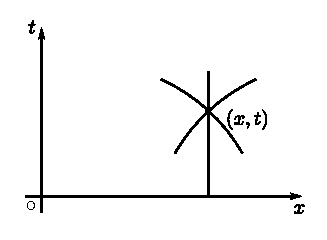
\includegraphics{figures/fig52-2.1.eps}
\caption{}\label{c1:fig2.1}
\end{figure}\pageoriginale

\begin{remark}\label{chap2:rem2.4}
In the fluid dynamic case the equations are non-linear and we cannot
know beforehand the characteristic values. However, their signs are
known and these already give some insight into the properties of the
solution. 
\end{remark}

\setcounter{exercise}{0}
\begin{exercise}\label{chap2:exer2.1}
Perform the same analysis in the Eulerian framework and show that the
eigenvalues are $u$, $u \pm C$.
\end{exercise}

\begin{remark}\label{chap2:rem2.5}
In fact the characteristics in the $m-t$ plane are defined by
$$
\frac{dm}{ds} = \lambda ; \; \frac{dt}{ds} = 1.
$$
In the $x-t$ plane, the images of the characteristic curves will be
the curves
$$
x = x (m(s), \; t(s)); \; t = t(s),
$$
and 
\begin{gather*}
\frac{dx}{ds} = \frac{\partial x}{\partial m} \; \frac{dm}{ds} +
\frac{\partial x}{\partial t} \; \frac{dt}{ds} =
\frac{J}{\rho_\circ} \lambda + u =\frac{\lambda}{\rho} + u\\
\frac{dt}{ds} = 1.
\end{gather*}
Hence the eigenvalues are $u$, $u\pm C$. 
\end{remark}

\begin{exercise}\label{chap2:exer2.2}
In\pageoriginale the euqations (\ref{eq2.16}), assuming we can integrate (iii)
to get $p$ in terms of $V$, we are then left with only two
equations. Thus for a perfect gas we get $pV^\gamma =a$ constant. For
the system (\ref{eq2.16}) (i) and (ii) in this case compute the eigenvalues
and eigen vectors. Find the Riemann invariant for each characteristic
curve. (They exist by virtue of remark \ref{chap2:rem2.2}).
\end{exercise}


\medskip
\noindent{\textbf{Reference.}}
The reader is referred to Courant and Friedrichs \cite{key9} for a
detailed exposition of characteristics of a hyperbolic system and
applications to hydrodynamic equations. 
